% -*- Mode:TeX -*-

%% IMPORTANT: The official thesis specifications are available at:
%%            http://libraries.mit.edu/archives/thesis-specs/
%%
%%            Please verify your thesis' formatting and copyright
%%            assignment before submission.  If you notice any
%%            discrepancies between these templates and the 
%%            MIT Libraries' specs, please let us know
%%            by e-mailing thesis@mit.edu

%% The documentclass options along with the pagestyle can be used to generate
%% a technical report, a draft copy, or a regular thesis.  You may need to
%% re-specify the pagestyle after you \include  cover.tex.  For more
%% information, see the first few lines of mitthesis.cls. 

%\documentclass[12pt,vi,twoside]{mitthesis}
%%
%%  If you want your thesis copyright to you instead of MIT, use the
%%  ``vi'' option, as above.
%%
%\documentclass[12pt,twoside,leftblank]{mitthesis}
%%
%% If you want blank pages before new chapters to be labelled ``This
%% Page Intentionally Left Blank'', use the ``leftblank'' option, as
%% above. 

\documentclass[12pt,vi]{mitthesis}
\usepackage[paper=a4paper,top=2.2cm, bottom=1.5cm, outer=1cm, inner=2.1cm]{geometry}% http://ctan.org/pkg/geometry
\usepackage{lgrind}
%% These have been added at the request of the MIT Libraries, because
%% some PDF conversions mess up the ligatures.  -LB, 1/22/2014
\usepackage{cmap}
\usepackage[T1]{fontenc}
%% Package "lmodern" added by user request see ServiceNow INC0396734 -OT, 4/29/2020
\usepackage{lmodern}
\pagestyle{plain}
\usepackage{tikz}
\usepackage{pdfoverlay}
\usepackage[ddmmyyyy]{datetime}
\renewcommand{\dateseparator}{.}
\usepackage{float}
\usepackage{xurl}
\usepackage{hyperref}
\usepackage{amsmath}
\usepackage{subcaption}
\usepackage{booktabs}
\usepackage{listings}
\usepackage{pifont}% http://ctan.org/pkg/pifont
\newcommand{\cmark}{\ding{51}}%
\newcommand{\xmark}{\ding{55}}%
\usetikzlibrary{positioning}

\def\abstract{
\vspace{5cm}
\begin{center}%
{\bfseries \abstractname\vspace{-.5em}}%
\end{center}
\quotation
}
\def\endabstract{\par
\endquotation
}

% Default fixed font does not support bold face
\DeclareFixedFont{\ttb}{T1}{txtt}{bx}{n}{12} % for bold
\DeclareFixedFont{\ttm}{T1}{txtt}{m}{n}{12}  % for normal

% Custom colors
\usepackage{color}
\definecolor{deepblue}{rgb}{0,0,0.5}
\definecolor{deepred}{rgb}{0.6,0,0}
\definecolor{deepgreen}{rgb}{0,0.5,0}

% Python style for highlighting
\newcommand\pythonstyle{\lstset{
language=Python,
basicstyle=\ttm,
otherkeywords={self},             % Add keywords here
keywordstyle=\ttb\color{deepblue},
emph={MyClass,__init__, modify, predict, explain_instance, append, concatenate, DataFrame, groupby, sort_values, as_list, , to_numeric, predict_proba, array, LimeTabularExplainer, fit, GaussianHMM, get_stationary_distribution, DecisionTreeClassifier},          % Custom highlighting
emphstyle=\ttb\color{deepred},    % Custom highlighting style
stringstyle=\color{deepgreen},
frame=tb,                         % Any extra options here
numbers = left,
breaklines,
xleftmargin = 15pt,
showstringspaces=false            % 
}}


% Python environment
\lstnewenvironment{python}[1][]
{
\pythonstyle
\lstset{#1}
}
{}

\begin{document}

\pagestyle{empty}
\pdfoverlaySetPDF{cover.pdf}
\begin{center}

{\large \textbf{PRACA DYPLOMOWA MAGISTERSKA}}
\vspace{6cm}

{\fontsize{18}{18}\selectfont \textbf{Hybrid neural networks for anomaly detection in~cyber-physical systems}}
\end{center}
\normalsize
\vspace{6cm}
\textbf{Wydział Fizyki Technicznej, Informatyki i Matematyki Stosowanej \\
Promotor:} dr hab. inż. Aneta Poniszewska-Marańda\\
\textbf{Dyplomant:} inż. Ramzi Hadrich\\
\textbf{Nr albumu:} 227488\\
\textbf{Kierunek:} Informatyka\\
\textbf{Specjalność:} Computer Science \& Information Technology\\
\begin{center}
    Łódź, \today r.
\end{center}


% First copy: start a new page, and save the page number.
\cleardoublepage
% Uncomment the next line if you do NOT want a page number on your
% abstract and acknowledgments pages.
\begin{abstract}
    My abstract
\end{abstract}


% Additional copy: start a new page, and reset the page number.  This way,
% the second copy of the abstract is not counted as separate pages.
% Uncomment the next 6 lines if you need two copies of the abstract
% page.
% \setcounter{page}{\thesavepage}
% \begin{abstractpage}
% \input{abstract}
% \end{abstractpage}

\cleardoublepage

\section*{Acknowledgements}

This is the acknowledgements section.  You should replace this with your
own acknowledgements.

%%%%%%%%%%%%%%%%%%%%%%%%%%%%%%%%%%%%%%%%%%%%%%%%%%%%%%%%%%%%%%%%%%%%%%
% -*-latex-*-


\pagestyle{plain}

\tableofcontents
\newpage
\listoffigures
\newpage
\listoftables

\chapter{Introduction} \label{chap:intro}

Cyber Physical Systems (CPS) are nowadays widely used in different application domains, such as smart-homes, smart-cities, hospitals, etc... They are mainly composed of two entities: a cyber part consisting in a computing and networking component, and a physical part consisting in different controllers and sensors. The existence of a connected cyber part implies its susceptibility to multiple cyber threats. The malfunctioning of these systems, due to a cyber threat, can cause severe impacts on the real life and the safety of the community, for example a blackout or water contamination. That is why many algorithms have been designed for the security monitoring of those systems, in particular the anomaly and attack detection.

Nowadays, machine and deep learning algorithms are used to detect those anomalies and intrusions. But, in majority, they rely only on the cyber part of the systems and on the data describing their behaviour, ignoring their physical models. The idea behind this work is to employ a hybrid machine learning algorithm, in particular neural networks, to detect anomalies and attacks in CPS considering its physical model.

In order to focus on the implementation of the hybrid machine learning algorithm, a CPS, with ready to use datasets, was chosen from a list provided in \cite{morris_industrial_nodate}: the power system \cite{adhikari_power_2014}, which network diagram was represented on figure \ref{fig:cps_rep}. The system is composed of two power generators who are alimenting the whole system. Intelligent Electronic Devices (IEDs) R1 to R4 and the breakers BR1 to BR4 can be found connected directly to those generators. Each IED switches its corresponding breaker when a fault is detected, valid or fake. The communication between the IEDs and the Substation Switch is done wirelessly. On the other hand the Substation Switch is connected with the Primary Domain Controller (PDC) and the Control Room.

\begin{figure}[H]
    \centering
    \includegraphics[width=100mm]{images/cps_rep.png}
    \caption{Power system network diagram \cite{adhikari_power_2014}}
    \label{fig:cps_rep}
\end{figure}

As mentioned before, the aim of the work is to fuse the black-box and theory-based models together to get better predictions. However this is not the first time such a fusion is examined. In the literature various approaches of the fusion of neural networks with theory-based models were presented. Those approaches can be divided into two types given what aspect of the algorithm they're changing: those that modify in first place the input to take into consideration the physical constraints, and those that modify the structure of the neural network.

-->here comes some more explanations--<

In the following chapters, it was decided to start with a less complex algorithms than neuron networks, so that the interpretation would be a lot simpler, in order to generalise the findings on the neural networks in further chapters. That is why the next chapter will talk about comparing some basic machine learning methods.
\section{Case study}
In order to focus on the implementation of the hybrid machine learning algorithm, a CPS, with ready to use datasets, was chosen from a list provided in \cite{morris_industrial_nodate}: the \textbf{power system} \cite{adhikari_power_2014}, which network diagram was represented on figure \ref{fig:cps_rep}. The system is composed of two power generators who are alimenting the whole system. Intelligent Electronic Devices (IEDs) R1 to R4 and the breakers BR1 to BR4 can be found connected directly to those generators. Each IED switches its corresponding breaker when a fault is detected, valid or fake. The communication between the IEDs and the Substation Switch is done wirelessly. On the other hand the Substation Switch is connected with the Primary Domain Controller (PDC) and the Control Room.

\begin{figure}[H]
    \centering
    \includegraphics[width=100mm]{images/cps_rep.png}
    \caption[Power system network diagram]{Power system network diagram \cite{adhikari_power_2014}}
    \label{fig:cps_rep}
\end{figure}

The operation of this power system can be described following 6 main scenarios:
\begin{itemize}
    \item normal behaviour, 
    \item short-circuit,
    \item line maintenance,
    \item remotely opening the breakers (attack),
    \item disruption of fault protection system (attack),
    \item fault imitation (attack).
\end{itemize} 
Each of those scenarios can be divided into several sub-scenarios concerning different entities of the system or/and the failure range. Every scenario was labelled with a number between 1 and 41. In this way \textbf{37 scenarios} are obtained, divided and numbered as follows:
\begin{itemize}
    \item 1 no events scenario, its number it is 41,
    \item 8 natural fault scenarios, its number ranges are 1-6 (short-circuit) and 13-14 (line maintenance),
    \item 28 attack scenarios, its number ranges are 7-12 (fault imitation), 15-20 (remotely opening the breakers), 20-30 and 35-40 (disruption of fault protection system).
\end{itemize}
The reason for dropping the numbers between 31 and 34 in the naming process of scenarios is not known.

The datasets provided in \cite{morris_industrial_nodate} represent \textbf{78377 events}, in which one of those scenarios was reproduced in the system. They have been grouped by scenario into 3 datasets: binary (attack or normal operation), three-class (attack, normal fault and no events) and multiclass (differentiating all 37 scenarios). Each of these 3 datasets is composed of 15 .arff or .csv files comporting in average 141 events for each of 37 scenarios. The exact number of events per file for each scheme is illustrated on figure \ref{fig:scen_distro_37}. For the 3 class dataset \textbf{55663 attack}, \textbf{18309 natural fault} and \textbf{4405 normal operation} events were found. The distribution of these schemes throughout the files is shown on figure~\ref{fig:scen_distro_file}. 

\begin{figure}[H]
    \centering
    \includegraphics[]{images/distr_allscen.pdf}
    \caption{Scenarios distribution throughout all 15 files} \label{fig:scen_distro_37}
\end{figure}

\begin{figure}[H]
    \centering
    \includegraphics[]{images/distr_3classes.pdf}
    \caption{Scenarios distribution throughout the 3-class dataset files}
    \label{fig:scen_distro_file}
\end{figure}

Figure \ref{fig:scen_distro_file} shows also this distribution for the binary datasets, it is sufficient to add the number of natural (orange) and normal operation (green) events.

The scenarios are not equally distributed in the case of the 37 schemes dataset, it is especially shown by the standard deviation of 61, which is an important value compared to some scenarios counting less than 100 events. On the other hand, in the case of 3-class scenarios, the distribution is even more not equal compared to the 37 schemes dataset. The \textbf{mean standard deviation among all files is equal to 1767}, which is an enormous result given that some scenarios count only around 100 events.

Each of previously mentioned events is described by \textbf{128 features}: 116 provided by four phasor measurement units\footnote{Phasor measurement units measure the electrical waves on an electricity grid} (each one provides 29 types of measurements) and 12 other features are reserved for control panel logs, snort alerts, relay logs of 4 phasors. The mentioned 116 features, each has a label formed by \textbf{concatenation} of the \textbf{source phasor reference} (it can be R1, R2, R3, R4) and the \textbf{measurement name}, as provided in table \ref{tab:pmu_mes}. For example R4-PM5:I stands for phase B current phase magnitude measured by R4.
%give exemple - preciser plus les features 
%expliquer les features plus
%figure pour explication de phase, magnitude

\begin{table}[H]
    \centering
    \caption[Phasor measurements]{Phasor measurements \cite{adhikari_power_2014}} \label{tab:pmu_mes}
    \begin{tabular}{lr}
        \toprule
        Feature&Description \\
        \midrule
        PA1:VH – PA3:VH&Phase A-C Voltage Phase Angle \\
        PM1:V – PM3:V&Phase A-C Voltage Phase Magnitude \\
        PA4:IH – PA6:IH&Phase A-C Current Phase Angle \\
        PM4:I – PM6:I&Phase A-C Current Phase Magnitude \\
        PA7:VH – PA9:VH&Pos.–Neg.– Zero Voltage Phase Angle \\
        PM7:V – PM9:V&Pos.–Neg.–Zero Voltage Phase Magnitude \\
        PA10:VH - PA12:VH&Pos.–Neg.–Zero Current Phase Angle \\
        PM10:V - PM12:V&Pos.–Neg.–Zero Current Phase Magnitude \\
        F&Frequency for relays \\
        DF&Frequency Delta (dF/dt) for relays \\
        PA:Z&Appearance Impedance for relays \\
        PA:ZH&Appearance Impedance Angle for relays \\
        S&Status Flag for relays \\
        \bottomrule
    \end{tabular}
\end{table} 

Those datasets have been used in several works related to CPS cyber-attack classification, one of which is \cite{borges_hink_machine_2014-1}, where the author try to find the most accurate algorithm to predict the status of the power system. The following chapter shows an attempt to partially reproduce the results obtained by them.

\chapter{Machine learning algorithms comparison} \label{chap:methods}

%essayer d'autres noyaux pour SVM
%roc pour tous les scenariaux
%concatenate all datasets

Before going further and analysing neural networks, a deeper look at classical machine learning algorithms will be taken, in particular Random Forest and Support Vector Machine (SVM) in the context of anomaly detection in the CPS presented in chapter \ref{chap:intro}. However this was done before in \cite{borges_hink_machine_2014-1} using the black-box model algorithms only. In their approach they used Weka \cite{witten_appendix_2017} in order to find the most performant algorithm among 7 they have chosen (OneR, NNge, Random Forest, Naïve Bayes, SVM, JRipper, Adaboost). 

This chapter shows an attempt to reproduce the results provided in \cite{borges_hink_machine_2014-1}, using two different machine learning toolkits (Weka and scikit-learn \cite{pedregosa_scikit-learn_2011}) in order to confirm the obtained results. That is why, first, these two toolkits will be presented, then the obtained results will be discussed.  

\section{Weka} \label{sec:weka_in_chap:methods}
%les parametres des algos, m par defaut
\textbf{Weka}, or more exactly \textbf{W}aikato \textbf{E}nvironment for \textbf{K}nowledge \textbf{A}nalysis, is an open source machine learning software developed at The University of Waikato in Hamilton, New Zealand and based on Java programming language. It is well known especially in academic environments and a lot of machine learning researches were conducted using it, one of them the mentioned before \cite{borges_hink_machine_2014-1}. It incorporates various machine learning tools: classifiers, regressors, visualizers, data pre-processor etc...

Weka is characterised by 3 main operating schemes. First, it can be run using a \textbf{graphical user interface} (GUI), enabling the user, even without deep knowledge in programming, to make machine learning experiments and analyse available classifiers. Second, more advanced users have the option to run all the available tools using a \textbf{command line}. Finally, Weka's tools can be \textbf{integrated directly into code in several programming languages (Java, Python, R, Spark)}, which enables even larger versatility.

\section{scikit-learn}
scikit-learn is an open-source machine learning \textbf{Python library} developed originally by David Cournapeau as a Google Summer of Code project and now it is maintained by a team of volunteers. It is well known in both academic and commercial environments, since it is used by many enterprises such as Spotify, Evernote, Booking.com, and research facilities like Inria or Télécom ParisTech \cite{noauthor_who_nodate}. It includes, just like Weka, various machine learning tools such as classifiers, regressors, data pre-processor etc... Its visualisation capabilities are limited, however there exist many additional Python packages for data visualisation such as YellowBrick, Eli5 and others... They will be further discussed in next chapter.

scikit-learn can be used only as an extension of Python language, what makes a bit harder for non experts to start working with it. However, since Python is an user friendly programming language and scikit-learn has a well made documentation, this toolkit is easy to use. Along with other Python packages, and especially pandas, scikit-learn is a very powerful, ergonomic and versatile solution for machine learning problems.  

It might be also interesting to mention that scikit-learn can be used within Weka after installing the appropriate add-on. This enables Weka users to use scikit-learn classifiers and regressors and run Python code just inside Weka's GUI.

\section{Metrics for classifiers comparison}
After the presentation of the used toolkits, in order to be able to compare machine learning algorithms the following metrics are introduced:
\begin{itemize}
    \item \textbf{accuracy}: ratio of correct classifications over the total number of samples,
    \item \textbf{precision}:  ratio of correct classifications for a particular class over all classifications that indicated that class,
    \item \textbf{recall}: ratio of correct classifications for a particular class, over all samples corresponding for this class,
    \item \textbf{f-measure}: weighted average of precision and recall given by the equation: 
    \begin{equation*}
        \text{f-measure} = 2 \times \frac{\mathrm{precision} \times \mathrm{recall}}{\mathrm{precision} + \mathrm{recall}}.
    \end{equation*}
\end{itemize}

In addition to that, precision, recall and f-measure metrics, can be calculated in three different ways:

\begin{itemize}
    \item \textbf{micro}: the metrics are determined globally by calculating true positives, false negatives and false positives,
    \item \textbf{macro}: the metrics are calculated for each class, then it gives their unweighted mean value,
    \item \textbf{weighted}: the metrics are calculated for each class, then it gives their weighted average value by the number of true instances for each class.
\end{itemize}

\section{Experimental setup}
In order to reproduce the results presented in \cite{borges_hink_machine_2014-1}, Weka version 3.8.4 and scikit-learn version 0.23.1, running on Anaconda 3.18.11 with Python 3.7.6.final.0, were used. Given the availability of classifiers between these two toolkits, only 3 classifiers were chosen: SVM, NaïveBayes and Random Forest. SVM in Weka comes from a package untitled libsvm available for this toolkit. The used parameters are presented for both scikit-learn and Weka in tables \ref{tab:sklearn_params} and \ref{tab:weka_params} respectively in order to help in the reproduction of this work in the features. For more information about particular parameters the references to their explanation are given in square-brackets next to each classifier.

\begin{table}[H]
    \caption{Scikit-learn classifiers parameters} \label{tab:sklearn_params}
    \scriptsize
    \centering
    \begin{subtable}[t]{.33\linewidth}
        \caption{Random Forest \cite{noauthor_sklearnensemblerandomforestclassifier_nodate}}
        \centering
        \begin{tabular}{lr}\toprule
            Parameter & Value \\\midrule
            n\_estimators & 100 \\
            criterion & "gini" \\
            max\_depth & None \\
            min\_samples\_split & 2 \\
            min\_samples\_leaf & 1 \\
            min\_weight\_fraction\_leaf & 0.0 \\
            max\_features & "log2" \\
            max\_leaf\_nodes & None \\
            min\_impurity\_decrease & 0.0 \\
            min\_impurity\_split & None \\
            bootstrap & True \\
            oob\_score & False \\
            n\_jobs & None \\
            random\_state & None \\
            verbose & 0 \\
            warm\_start & False \\
            class\_weight & None \\
            ccp\_alpha & 0.0 \\
            max\_samples & None \\\bottomrule
        \end{tabular}
    \end{subtable}%
    \begin{subtable}[t]{.35\linewidth}
        \caption{SVM \cite{noauthor_sklearnsvmsvc_nodate}}
        \centering
        \begin{tabular}{lr}\toprule
            Parameter & Value \\\midrule
            C & 1.0 \\
            kernel & "rbf" \\
            degree & 3 \\
            gamma & "scale" \\
            coef0 & 0.0 \\
            shrinking & True \\
            probability & True \\
            tol & 1e-3 \\
            cache\_size & 7000 \\
            class\_weight & None \\
            verbose & False \\
            max\_iter & 1000 \\
            decision\_function\_shape & "ovr" \\
            break\_ties & False \\
            random\_state & None \\\bottomrule
        \end{tabular}
    \end{subtable}%
    \begin{subtable}[t]{.23\linewidth}
        \caption{NaïveBayes \cite{noauthor_sklearnnaive_bayesgaussiannb_nodate}}
        \centering
        \begin{tabular}{lr}\toprule
            Parameter & Value \\\midrule
            priors & None \\
            var\_smoothing & 1e-9 \\\bottomrule
        \end{tabular}
    \end{subtable}%
\end{table}


\begin{table}[H]
    \caption{Weka classifiers parameters} \label{tab:weka_params}
    \scriptsize
    \centering
    \begin{subtable}[t]{.37\linewidth}
        \caption{Random Forest \cite{noauthor_randomforest_nodate}}
        \centering
        \begin{tabular}{lr}\toprule
            Parameter & Value \\\midrule
            bagSizePercent & 100\\
            batchSize & 100 \\
            breakTiesRandomly & False \\
            calcOutOfBag & False \\
            computeAttributeImportance & False \\
            debug & False \\
            doNotCHeckCapabilities & False \\
            maxDepth & 0 \\
            numDecimalPlaces & 2 \\
            numExecutionSlots & 1 \\
            numFeatures & 0 \\
            numIterations & 100 \\
            outputOutOfBagComplexityStatistics & False \\
            printClassifiers & False \\
            seed & 1 \\
            storeOutOfBagPredictions & False \\\bottomrule
        \end{tabular}
    \end{subtable}%
    \begin{subtable}[t]{.37\linewidth}
        \caption{SVM \cite{noauthor_libsvm_nodate}}
        \centering
        \begin{tabular}{lr}\toprule
            Parameter & Value \\\midrule
            SVMType & C-SVC (classification) \\
            batchSize & 100 \\
            cacheSize & 40.0 \\
            coef0 & 0.0 \\
            cost & 1.0 \\
            debug & False \\
            degree & 3 \\
            doNotCHeckCapabilities & False \\
            doNotReplaceMissingValues & False \\
            eps & 0.001 \\
            gamma & 0.0 \\
            kernelType & radial basis function\\
            loss & 0.1 \\
            modelFile & Weka-3-8-4 \\
            normalize & False \\
            nu & 0.5 \\
            numDecimalPlaces & 2 \\
            probabilityEstimates & False \\
            seed & 1 \\
            shrinking & True \\
            weights & \\\bottomrule
        \end{tabular}
    \end{subtable}%
    \begin{subtable}[t]{0.385\linewidth}
        \caption{NaïveBayes \cite{noauthor_naivebayes_nodate}}
        \centering
        \begin{tabular}{lr}\toprule
            Parameter & Value \\\midrule
            batchSize & 100 \\
            debug & False \\
            displayModelInOldFormat & False \\
            doNotCHeckCapabilities & False \\
            numDecimalPlaces & 2 \\
            useKernelEstimator & False \\
            useSupervisedDiscretization & False\\\bottomrule
        \end{tabular}
    \end{subtable}%
\end{table}

% \includegraphics{/images/weka/randomforest.png}
% \includegraphics{/images/weka/nb.png}
% \includegraphics{/images/weka/svm.png}
\section{Comparison results}


\begin{figure}[H]
    \centering
    \begin{subfigure}[t]{0.5\textwidth}
        \includegraphics[width=\linewidth]{images/weka_accuracy3}
        \caption{Our attempt}
    \end{subfigure}%
    \begin{subfigure}[t]{0.5\textwidth}
        \includegraphics[width=\linewidth]{images/weka_accuracy3_cite.png}
        \caption{Original results \cite{borges_hink_machine_2014-1}}
    \end{subfigure}
    \caption{Accuracy for three-class datasets}
    \label{fig:weka_acc3}
\end{figure}

\begin{figure}[H]
    \centering
    \begin{subfigure}[t]{0.5\textwidth}
        \includegraphics[width=\linewidth]{images/weka_accuracy2}
        \caption{Our attempt}
    \end{subfigure}%
    \begin{subfigure}[t]{0.5\textwidth}
        \includegraphics[width=\linewidth]{images/weka_accuracy2_cite.png}
        \caption{Original results \cite{borges_hink_machine_2014-1}}
    \end{subfigure}
    \caption{Accuracy for binary datasets}
    \label{fig:weka_acc2}
\end{figure}

\begin{figure}[H]
    \centering
    \begin{subfigure}[t]{0.5\textwidth}
        \includegraphics[width=\linewidth]{images/weka_accuracyall}
        \caption{Our attempt}
    \end{subfigure}%
    \begin{subfigure}[t]{0.5\textwidth}
        \includegraphics[width=\linewidth]{images/weka_accuracyall_cite.png}
        \caption{Original results \cite{borges_hink_machine_2014-1}}
    \end{subfigure}
    \caption{Accuracy for multiclass datasets}
    \label{fig:weka_accall}
\end{figure}

\begin{figure}[H]
    \centering
    \begin{subfigure}[t]{0.5\textwidth}
        \includegraphics[width=\linewidth]{images/weka_precision}
        \caption{Our attempt}
    \end{subfigure}%
    \begin{subfigure}[t]{0.5\textwidth}
        \includegraphics[width=\linewidth]{images/weka_precision_cite.png}
        \caption{Original results \cite{borges_hink_machine_2014-1}}
    \end{subfigure}
    \caption{Precision}
    \label{fig:weka_prec}
\end{figure}

\begin{figure}[H]
    \centering
    \begin{subfigure}[t]{0.5\textwidth}
        \includegraphics[width=\linewidth]{images/weka_recall}
        \caption{Our attempt}
    \end{subfigure}%
    \begin{subfigure}[t]{0.5\textwidth}
        \includegraphics[width=\linewidth]{images/weka_recall_cite.png}
        \caption{Original results \cite{borges_hink_machine_2014-1}}
    \end{subfigure}
    \caption{Recall}
    \label{fig:weka_recall}
\end{figure}

\begin{figure}[H]
    \centering
    \begin{subfigure}[t]{0.5\textwidth}
        \includegraphics[width=\linewidth]{images/weka_f1}
        \caption{Our attempt}
    \end{subfigure}%
    \begin{subfigure}[t]{0.5\textwidth}
        \includegraphics[width=\linewidth]{images/weka_f1_cite.png}
        \caption{Original results \cite{borges_hink_machine_2014-1}}
    \end{subfigure}
    \caption{F-measure}
    \label{fig:weka_f1}
\end{figure}

The obtained results indicate clearly that Random Forest algorithm is the more accurate and gives clearly the best results, with Adaboost+JRIP with slightly worse performance. On the other hand, the results presented in \cite{borges_hink_machine_2014-1} shows better results for Adaboost+JRIP. For SVM and Naïve Bayes the results are comparable, expect for precision value for SVM. The origin of this difference is so far unknown.

% In addition to the mentioned algorithms, the multiplayer perceptron algorithm (MLP) was used in order to have an initial idea on its performance. The obtained results show that it is less accurate than Random Forest and Adaboost+JRIP algorithms with an accuracy of approximatively 90\%, the values of precision and recall are respectively 0.8 and 0.65, which are good results.

% The results of classification analysis are shown on figure \ref{fig:scikit_results}. In contrast to Weka's result, precision, recall and f-measure indicators come with three different values:


\begin{figure}[H]
\centering
\begin{subfigure}[t]{0.475\textwidth}
    \centering
    \includegraphics[page=1, width=\linewidth]{images/results_scikit.pdf}
    \caption{Accuracy}
    \label{fig:scikit_accuracy}
\end{subfigure}
\begin{subfigure}[t]{0.475\textwidth}
    \centering
    \includegraphics[page=3, width=\linewidth]{images/results_scikit.pdf}
    \caption{Precision}
    \label{fig:scikit_prec}
\end{subfigure}
\caption{scikit-learn results}
\end{figure}
\begin{figure}[H]\ContinuedFloat
\begin{subfigure}[t]{0.475\textwidth}
    \centering
    \includegraphics[page=4, width=\linewidth]{images/results_scikit.pdf}
    \caption{Recall\footnote{micro and weighted values are the same in this case.}}
    \label{fig:scikit_recall}
\end{subfigure}
\begin{subfigure}[t]{0.475\textwidth}
    \centering
    \includegraphics[page=2, width=\linewidth]{images/results_scikit.pdf}
    \caption{F-measure}
    \label{fig:scikit_f1}
\end{subfigure}
\caption{scikit-learn results}
\label{fig:scikit_results}
\end{figure}

It can be observed that the obtained results are partially different from those obtained using Weka. The results for MLP and Naïve Bayes are comparable to those from Weka, but on the other hand, the results for Random Forest and SVM differ considerably. This made MLP the most reliable classifier compared to others in this comparison.

It can be also deducted that Weka is calculating metrics globally (corresponds to micro in scikit-learn).

\section{scikit-learn further methods' analysis}

In addition to all that, scikit-learn enables the user to plot the receiver operating characteristic (ROC) curves for each class and the confusion matrix. The ROC curve represents the plot od true positive rate when the false positive rate changes. The confusion matrix on the other hand shows the normalized number (over the total number of samples) of predicted values of each class for each class. The results are illustrated on figures \ref{fig:ROCCM_RF}, \ref{fig:ROCCM_SVM}, \ref{fig:ROCCM_NB} and \ref{fig:ROCCM_MLP}.

\begin{figure}[H]
    \begin{subfigure}[t]{0.45\textwidth}
        \centering
        \includegraphics[page=1, width=\linewidth]{images/results_scikit/RandomForest}
        \caption{ROC Curve}
        \label{fig:scikit_RF_ROC}
    \end{subfigure}
    \begin{subfigure}[t]{0.45\textwidth}
        \centering
        \includegraphics[page=2, width=\linewidth, trim= 0 50 0 100, clip]{images/results_scikit/RandomForest}
        \caption{Confusion Matrix}
        \label{fig:scikit_RF_CM}
    \end{subfigure}
    \caption{Random Forest ROC curve and confusion matrix}
    \label{fig:ROCCM_RF}
\end{figure}

\begin{figure}[H]
    \begin{subfigure}[t]{0.45\textwidth}
        \centering
        \includegraphics[page=1, width=\linewidth]{images/results_scikit/SVM}
        \caption{ROC Curve}
        \label{fig:scikit_SVM_ROC}
    \end{subfigure}
    \begin{subfigure}[t]{0.45\textwidth}
        \centering
        \includegraphics[page=2, width=\linewidth, trim= 0 50 0 100, clip]{images/results_scikit/SVM}
        \caption{Confusion Matrix}
        \label{fig:scikit_SVM_CM}
    \end{subfigure}
    \caption{SVM ROC curve and confusion matrix}
    \label{fig:ROCCM_SVM}
\end{figure}

\begin{figure}[H]
    \begin{subfigure}[t]{0.45\textwidth}
        \centering
        \includegraphics[page=1, width=\linewidth]{images/results_scikit/NaiveBayes}
        \caption{ROC Curve}
        \label{fig:scikit_NB_ROC}
    \end{subfigure}
    \begin{subfigure}[t]{0.45\textwidth}
        \centering
        \includegraphics[page=2, width=\linewidth, trim= 0 50 0 100, clip]{images/results_scikit/NaiveBayes}
        \caption{Confusion Matrix}
        \label{fig:scikit_NB_CM}
    \end{subfigure}
    \caption{Naïve Bayes ROC curve and confusion matrix}
    \label{fig:ROCCM_NB}
\end{figure}

\begin{figure}[H]
    \begin{subfigure}[t]{0.45\textwidth}
        \centering
        \includegraphics[page=1, width=\linewidth]{images/results_scikit/MLP}
        \caption{ROC Curve}
        \label{fig:scikit_MLP_ROC}
    \end{subfigure}
    \begin{subfigure}[t]{0.45\textwidth}
        \centering
        \includegraphics[page=2, width=\linewidth, trim= 0 50 0 100, clip]{images/results_scikit/MLP}
        \caption{Confusion Matrix}
        \label{fig:scikit_MLP_CM}
    \end{subfigure}
    \caption{MLP ROC curve and confusion matrix}
    \label{fig:ROCCM_MLP}
\end{figure}

The previous figures show that Random Forest classifier has the higher capacities to distinguish between the occurrence of each class, or it's absence. It's visible on both ROC curve and the confusion matrix, where the highest number of predictions is shown for the true positives for each class. SVM tends to predict only NoEvents and Attacks but does not really succeed in distinguishing between them. Naïve Bayes fails to make true predictions, it considers everything of class natural. Finally MLP, it succeeds in determining the class NoEvents, but does not distinguish over classes almost at all, despite the high accuracy (it is due because of the huge number of samples of class NoEvents).

Given this analysis, it can be deducted that Random Forest algorithm acts the best, and that is why it will be adapted in next chapters, in which, at first, an analysis of features and their importance will be made. However a deeper look at the amelioration of MLP will be also made later.


\chapter{Features' importance}

After having determined the most performant algorithm, which is Random Forest, it is time to go further and analyse which features impact the results of classification the most. In order to do that, six tools will be examined: Lime \cite{lime}, ELI5 \cite{mikhail_korobov_eli5_nodate}, YellowBrick \cite{bengfort_yellowbrick_2018}, Treeinterpreter \cite{ando_saabas_treeinterpreter_nodate}, dtreeviz \cite{terence_parr_dtreeviz_nodate} and export\_graphviz tool from scikit-learn, where the last three ones are designed for Random Forest and Decison Tree classifiers.

However, before going deeper into features' importance classification, the features itself should be discussed. The power system presented \cite{adhikari_power_2014} is described by 128 features: 116 provided by four phasor measurement units\footnote{Phasor measurement units measure the electrical waves on an electricity grid} (each one provides 29 types of measurements) and 12 other features are reserved for control panel logs, snort alerts, relay logs of 4 phasors. The mentioned 116 features, each has a label formed by concatenation of the source phasor reference (it can be R1, R2, R3, R4) and the measurement name, as provided in table \ref{tab:pmu_mes}.

\begin{table}[H]
    \centering
    \caption[Phasor measurements]{Phasor measurements \cite{adhikari_power_2014}} \label{tab:pmu_mes}
    \begin{tabular}{|c|c|}\hline
        \textbf{Feature}&\textbf{Description} \\\hline
        PA1:VH – PA3:VH&Phase A - C Voltage Phase Angle \\\hline
        PM1: V – PM3: V&Phase A - C Voltage Phase Magnitude \\\hline
        PA4:IH – PA6:IH&Phase A - C Current Phase Angle \\\hline
        PM4: I – PM6: I&Phase A - C Current Phase Magnitude \\\hline
        PA7:VH – PA9:VH&Pos. – Neg. – Zero Voltage Phase Angle \\\hline
        PM7: V – PM9: V&Pos. – Neg. – Zero Voltage Phase Magnitude \\\hline
        PA10:VH - PA12:VH&Pos. – Neg. – Zero Current Phase Angle \\\hline
        PM10: V - PM12: V&Pos. – Neg. – Zero Current Phase Magnitude \\\hline
        F&Frequency for relays \\\hline
        DF&Frequency Delta (dF/dt) for relays \\\hline
        PA:Z&Appearance Impedance for relays \\\hline
        PA:ZH&Appearance Impedance Angle for relays \\\hline
        S&Status Flag for relays \\\hline
    \end{tabular}
\end{table}

\section{Lime}
Lime is a tool that is used to explain the behaviour of machine learning classifiers. It supports, as for this day, only the explanation of individual predictions. As output it gives a list of features ordered by their relative importance in the prediction of this particular sample.

In order to class the features according to their importance, Lime approximates the model by an interpretable one, created based on perturbing the features of the examined instance. More the perturbed instances are similar to the examined instance, higher is the weight that gets the perturbed feature.

Since in this case the explanations of single samples are not really interesting, an attempt to generalize the results was made: Lime explainer was run on 100 false predictions of a chosen class. The results are concatenated together, and for all the features that are duplicated, the importance is calculated as the mean value of the importances and only one entry is kept with the calculated average importance. This algorithm was also run omitting the differentiation between classes. The results, reduced to 10 entries each, are shown below.

For NoEvents class:
\begin{verbatim}
                                     importance
 feature                                      
 R2-PM1:V > 130872.03                -0.013013
 R3-PA2:VH <= -93.75                 -0.011134
 R2-PA7:VH <= -101.20                -0.010218
 R3-PM2:V > 130431.15                -0.009583
 R2-PM7:V > 130857.40                -0.009377
 ...                                       ...
 R3-PM5:I <= 330.70                   0.005762
 0.00 < R1-PA12:IH <= 32.04           0.007514
 128762.21 < R2-PM1:V <= 129859.49    0.007776
 R3-PM2:V <= 128425.29                0.007998
 R4-PA5:IH > 115.38                   0.008534
 
 [361 rows x 1 columns]
\end{verbatim}

For Attack class:
\begin{verbatim}
                                   importance
    feature                                 
    R3-PA2:VH > 113.97             -0.012837
    -97.10 < R4-PA7:VH <= -35.66   -0.010994
    -97.43 < R1-PA7:VH <= -35.85   -0.010306
    R2-PA2:VH > 114.00             -0.009730
    R3-PM2:V <= 128425.29          -0.006914
    ...                                  ...
    R3-PA2:VH <= -93.75             0.008307
    R3-PA7:VH <= -101.22            0.008676
    R2-PM1:V > 130872.03            0.009242
    R3:S > 0.00                     0.010717
    R2-PA7:VH <= -101.20            0.014018
    
    [380 rows x 1 columns]
\end{verbatim}

For Natural class: 
\begin{verbatim}
                            importance
    feature                          
    R2-PA5:IH <= -74.26     -0.003613
    R4-PM3:V > 132484.78    -0.002835
    R4-PM2:V > 132187.18    -0.002437
    R2-PM7:V <= 128751.24   -0.002290
    R2-PM1:V <= 128762.21   -0.002151
    ...                           ...
    R1-PA1:VH > 71.28        0.003518
    R2-PM7:V > 130857.40     0.003693
    R2-PA5:IH > 63.30        0.004103
    R3:F > 60.00             0.004873
    R2:F > 60.00             0.005168
    
    [331 rows x 1 columns]]
\end{verbatim}

For all classes:
\begin{verbatim}
                                 importance
    feature                                
    R3-PM2:V <= 128425.29         -0.006715
    R2-PA7:VH > 65.91             -0.006353
    R3-PM5:I <= 330.70            -0.006009
    -40.44 < R3-PA1:VH <= 65.76   -0.005808
    R3-PA4:IH <= -65.22           -0.005764
    ...                                 ...
    R2-PA3:VH <= -75.28            0.005588
    R3-PA4:IH > 102.49             0.005723
    R4-PA1:VH > 71.50              0.007481
    R3-PM2:V > 130431.15           0.008501
    R2-PM1:V > 130872.03           0.009070
    
    [331 rows x 1 columns]
\end{verbatim}
\section{ELI5}

\section{YellowBrick}

\section{Random Forest and Decision Trees}
\subsection{Treeinterpreter}

\subsection{dtreeviz}

\subsection{scikit-learn export\_graphviz}
\chapter{Model enhancement}
After having chosen the appropriate machine learning algorithms and found a way to determine the most important features in the classification problem, this chapter is an attempt to create a model able to enhance the results obtained by the basic classification. Three different approaches are presented. First of all, the most important features values were altered and the effect of this modification is examined. Second, a formula for calculating the distance between different samples is established then a way to use that information. Finally, the Hidden Markov Models were used in order to determine the likeliness of prediction of a particular class and this data was used to modify the machine learning algorithm. 

\section{Features values modification}
The first proposed solution considers changing the values of most important features in the dataset after the training process. In other words the training process occurs normally, then the importances are determined and a correction function is created (figure \ref{fig:train}). This correction function will act then on the samples introduced to the model in order to change the features values and obtain better predictions (figure \ref{fig:predict}). 

\begin{figure}[H]
    \centering
    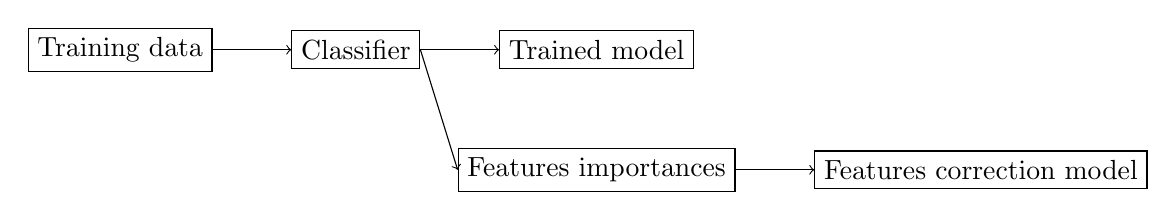
\begin{tikzpicture}
        \node[rectangle, draw=black] (main) {Training data};
        \node[rectangle, draw=black] (DecisionTree) [right=of main] {Classifier};
        \node[rectangle, draw=black] (out1) [right=of DecisionTree] {Trained model};
        \node[rectangle, draw=black] (out2) [below=of out1] {Features importances};
        \node[rectangle, draw=black] (feat) [right=of out2] {Features correction model};
   
        \draw[->] (main.east) -- (DecisionTree.west);
        \draw[->] (DecisionTree.east) -- (out1.west);
        \draw[->] (DecisionTree.east) -- (out2.west); 
        \draw[->] (out2.east) -- (feat.west);
    \end{tikzpicture}
    \caption{Training process illustration} \label{fig:train}
\end{figure}

\begin{figure}[H]
    \centering
    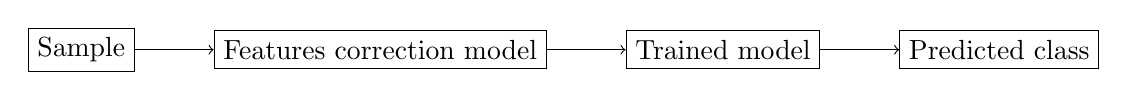
\begin{tikzpicture}
        \node[rectangle, draw=black] (main) {Sample};
        \node[rectangle, draw=black] (correl) [right=of main] {Features correction model};
        \node[rectangle, draw=black] (model) [right=of correl] {Trained model};
        \node[rectangle, draw=black](out) [right=of model] {Predicted class};

        \draw[->] (main.east) -- (correl.west);
        \draw[->] (correl.east) -- (model.west);
        \draw[->] (model.east) -- (out.west);
    \end{tikzpicture}
    \caption{Prediction illustration} \label{fig:predict}
\end{figure}

\section{Distance between features}


\section{Hidden Markov Models}


\chapter{Conclusions}

The aim of this thesis was to develop a hybrid neural network capable of differentiating between three states of a cyber physical system - normal behaviour, a fault or an attack. To facilitate the work and focus on computer science topics, ready datasets for a power system was taken and analysed in chapter 2. 

The final obtained results do not provide a full answer for the provided aim, because they do not represent in fact hybrid neural network but a decision tree classifier. However, a decision tree classifier is still a machine learning technique and the obtained results may be generalized to the neural networks case.

It was found that the most effective way to enhance classification results was to create a new dataset combining the distance of the samples to the three classes with the values of the fifteen more important features. The other two described method were slightly less effective, especially the method where probabilities found by Hidden Markov Model were used. The inaccuracy of this last method may be explained by the time independence of the used datasets. Maybe using another dataset would ameliorate the results.

The increase of the values of the metrics was not very significant even with the best method. Maybe using a physical model of the power system that could estimate on its own some features and combine this with a machine learning technique would give better results. There exist some python toolkits created to model a power system like PyPSA \cite{brown_pypsapypsa_2020} or pandapower \cite{noauthor_pandapower_nodate}, but they are complex and require specific advanced technical skills.

This thesis in addition to all that, provides some other important conclusions. First, the different machine learning toolkits do not work always the same way and the results may differ from one toolkit to another, like in this case and the differences in results between Weka and scikit-learn. Second, in order to the results from a work to be reproductible, all the details concerning the used parameters and the version of the software must be provided, in other case it may be hard to get the same result. Finally, it exists plenty of tools for machine learning classifiers evaluation and each toolkit provides its own interpretation of results.

This work may be continued by implementing the power system using one of the mentioned toolkits in order to try to further enhance the results. In addition to that, instead of using scikit-learn, Keras \cite{noauthor_keras_nodate} or PyTorch \cite{noauthor_pytorch_nodate} packages may be used in order to create a complex neural network and possibly get better results.   

%\appendix

\cleardoublepage
\phantomsection
\addcontentsline{toc}{chapter}{Bibliography}
\bibliography{main}
\bibliographystyle{ieeetr}

\end{document}

